\documentclass[12pt,a4paper]{article}
\usepackage{amsmath,amscd,amsbsy,amssymb,latexsym,url,bm,amsthm}
\usepackage{epsfig,graphicx,subfigure}
\usepackage{enumitem,balance}
\usepackage{wrapfig}
\usepackage{mathrsfs,euscript}
\usepackage[usenames]{xcolor}
\usepackage{hyperref}
\usepackage[vlined,ruled,linesnumbered]{algorithm2e}
\usepackage{float}
\hypersetup{colorlinks=true,linkcolor=black}

\newtheorem{theorem}{Theorem}
\newtheorem{lemma}[theorem]{Lemma}
\newtheorem{proposition}[theorem]{Proposition}
\newtheorem{corollary}[theorem]{Corollary}
\newtheorem{exercise}{Exercise}
\newtheorem*{solution}{Solution}
\newtheorem{definition}{Definition}
\theoremstyle{definition}

\renewcommand{\thefootnote}{\fnsymbol{footnote}}

\newcommand{\postscript}[2]
{\setlength{\epsfxsize}{#2\hsize}
	\centerline{\epsfbox{#1}}}

\renewcommand{\baselinestretch}{1.0}

\setlength{\oddsidemargin}{-0.365in}
\setlength{\evensidemargin}{-0.365in}
\setlength{\topmargin}{-0.3in}
\setlength{\headheight}{0in}
\setlength{\headsep}{0in}
\setlength{\textheight}{10.1in}
\setlength{\textwidth}{7in}
\makeatletter \renewenvironment{proof}[1][Proof] {\par\pushQED{\qed}\normalfont\topsep6\p@\@plus6\p@\relax\trivlist\item[\hskip\labelsep\bfseries#1\@addpunct{.}]\ignorespaces}{\popQED\endtrivlist\@endpefalse} \makeatother
\makeatletter
\renewenvironment{solution}[1][Solution] {\par\pushQED{\qed}\normalfont\topsep6\p@\@plus6\p@\relax\trivlist\item[\hskip\labelsep\bfseries#1\@addpunct{.}]\ignorespaces}{\popQED\endtrivlist\@endpefalse} \makeatother

\begin{document}
	\noindent
	
	%========================================================================
	\noindent\framebox[\linewidth]{\shortstack[c]{
			\Large{\textbf{Lab05-DynamicProgramming}}\vspace{1mm}\\
			CS214-Algorithm and Complexity, Xiaofeng Gao, Spring 2021.}}
	\begin{center}
		\footnotesize{\color{red}$*$ If there is any problem, please contact TA Haolin Zhou.}
		
		% Please write down your name, student id and email.
		\footnotesize{\color{blue}$*$ Name:Renyang Guan  \quad Student ID:519021911058 \quad Email: guanrenyang@sjtu.edu.cn}
		
	\end{center}
	
	\begin{enumerate}
		\item \textit{Optimal Binary Search Tree.} Given a sorted sequence $K=\left \langle k_{1}, k_{2}, \ldots, k_{n} \right \rangle$ of $n$ distinct keys, and we wish to build a binary search tree from these keys. For each key $k_{i}$, we have a probability $p_{i}$ that a search will be for $k_{i}$. Some searches may be for values not in $K,$ and so we also have $n+1$ \emph{dummy keys} $d_{0}, d_{1}, d_{2}, \ldots, d_{n}$ representing values not in $K$. In particular, $d_{0}$ represents all values less than $k_{1}$, and $d_{n}$ represents all values greater than $k_{n}$. For $i=1,2, \ldots, n-1,$ the dummy key $d_{i}$ represents all values between $k_{i}$ and $k_{i+1}$. For each dummy key $d_{i}$, we have a probability $q_{i}$ that a search will correspond to $d_{i}$. Each key $k_{i}$ is an internal node, and each dummy key $d_{i}$ is a leaf. Every search is either successful (finding some key $k_{i}$ ) or unsuccessful (finding some dummy key $d_{i}$ ), and so we have $ \sum_{i=1}^{n} p_{i}+\sum_{i=0}^{n} q_{i}=1 $. 
		\begin{enumerate}
			\item Prove that if an optimal binary search tree $T$ ($ T $ has the smallest expected search cost) has a subtree $T^{\prime}$ containing keys $k_{i}, \ldots, k_{j},$ then this subtree $T^{\prime}$ must be optimal as well for the subproblem with keys $k_{i}, \ldots, k_{j}$ and dummy keys $d_{i-1}, \ldots, d_{j}$. 
			\item We define $e[i, j]$ as the expected cost of searching an optimal binary search tree containing the keys $k_{i}, \ldots, k_{j} .$ Our goal is to compute $e[1, n]$. Write the state transition equation and pseudocode using \textbf{dynamic programming} to find
			the minimum expected cost of a search in a given binary tree. (\textbf{Remark}: You may use $ w(i, j)=\sum_{l=i}^{j} p_{l}+\sum_{l=i-1}^{j} q_{l} $).
			\item Implement your proposed algorithm in C/C++ and analyze the time complexity. ({\color{blue}The framework Code-OBST.cpp is attached on the course webpage}). Give the minimum search cost calculated by your algorithm. The test case is given as following:
			\begin{table}[H]
				\setlength{\abovecaptionskip}{0cm}
				\setlength{\belowcaptionskip}{0.1cm}
				\centering		
				\begin{tabular}{|c|cccccccc|}
					\hline
					$ i $&0&1&2&3&4&5&6&7\\
					\hline
					$ p_{i} $&&0.04&0.06&0.08&0.02&0.10&0.12&0.14\\
					\hline
					$ q_{i} $&0.06&0.06&0.06&0.06&0.05&0.05&0.05&0.05\\
					\hline
				\end{tabular}
			\end{table}
			\item Please draw the structure of the optimal binary search tree in the test case, and explain the drawing process.   
		\end{enumerate}
		    \begin{solution}
		    ~\\
		        \begin{enumerate}
		            \item 
		            \begin{proof}
		            \textbf{\textit{Counter evidence:}} 
		            If the binary search tree $T$ is optimal, suppose that there exists a subtree $T''$ whose expected cost is smaller than $T'$. We could cut $T''$ and substitute $T'$ with $T''$ to make the total expected cost lower. Since the binary search tree $T$ is optimal, the substitution is impossible. 
		            \end{proof}
		            
		            \item\textbf{\textit{State transition equation:}}
		            \begin{equation}
		                e[i,j]=\begin{cases}
		                q_{i-1} & j=i-1\\
		                \mathop{min}\limits_{i\leq r\leq j}\{e[i,r-1]+e[r+1,j]+\omega (i,j)\} & i\leq j
		                \end{cases}
		            \end{equation}
		            
		            \begin{algorithm}[H]
		            \KwIn{$p,q,n$}
		            \KwOut{Array $e$, array $root$}
		            initialize three 2-dimentional arrays:\;
		            $e[1,\cdots,n+1][0,\cdots,n]$\;
		            $\omega [1,\cdots,n+1][0,\cdots,n]$\;
		            $root[1,\cdots,n][1,\cdots,n]$\;
		            \BlankLine
                    
                    \For{$i\leftarrow 1$ \KwTo $n+1$ }
                    {
                        $e[i,i-1]\leftarrow q_{i-1}$\;
                        $\omega [i,i-1]\leftarrow q_{i-1}$\;
                    }
                    
                    \For{$t\leftarrow 1$ \KwTo $n$}
                    {
                        \For{$i\leftarrow 1$\KwTo $n-t+1$}{
                        $j=i+t-1$\;
                        $e[i,j]\leftarrow \infty$\;
                        $\omega [i,j]=\omega [i,j-1] +p_j+q_j$\;
                        \For{$l=i$ \KwTo $j$}{
                            $temp\leftarrow e[i,t-1]+e[t+1,j]+\omega[i,j]$\;
                            \If{$temp\leq e[i,j]$}
                            {
                                $e[i,j]=temp$\;
                                $root[i,j]\leftarrow l$\;
                            }
                        }
                        }
                    }
		            \caption{Pseudocode of optimal binary search  tree}\label{Alg-OBST}
		            
		            \end{algorithm}
		            \item
		            The source code is shown in file \textit{Code-OBST.cpp}.
		            
		            \textbf{\textit{Result of the program:}}
        		    \begin{figure}[htbp]
                        \centering 
                        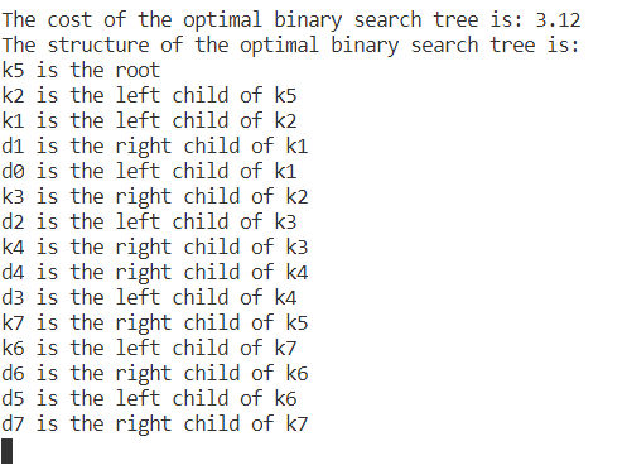
\includegraphics[width=0.6\textwidth]{Fig-Result1.pdf}
                        \caption{Program Result}\label{Fig-Result1}
                    \end{figure}
                    
		            \textbf{\textit{Time complexity analysis:}}
		            \\
		            \\
		            Assume that all the operations with time complexity $O(1)$ are represented by $1$ in the formula below.
		            $$Time\ complexity=n+1+\sum_{t=1}^n\sum_{i=1}^{n-t+1}t=n+1+\sum_{t=1}^n -t^2+(n+1)t=\frac{1}{6}n^3+\frac{1}{2}n^2+\frac{4}{3}n+1=\Omega(n^3)$$
		            
		            \textbf{\textit{The minimum search cost}} is \emph{$3.12$}.
		            
		            \item
		            The optimal binary search tree is shown in Fig.~\ref{Fig-Tree}:
		            
                    \begin{figure}[htbp]
                        \centering 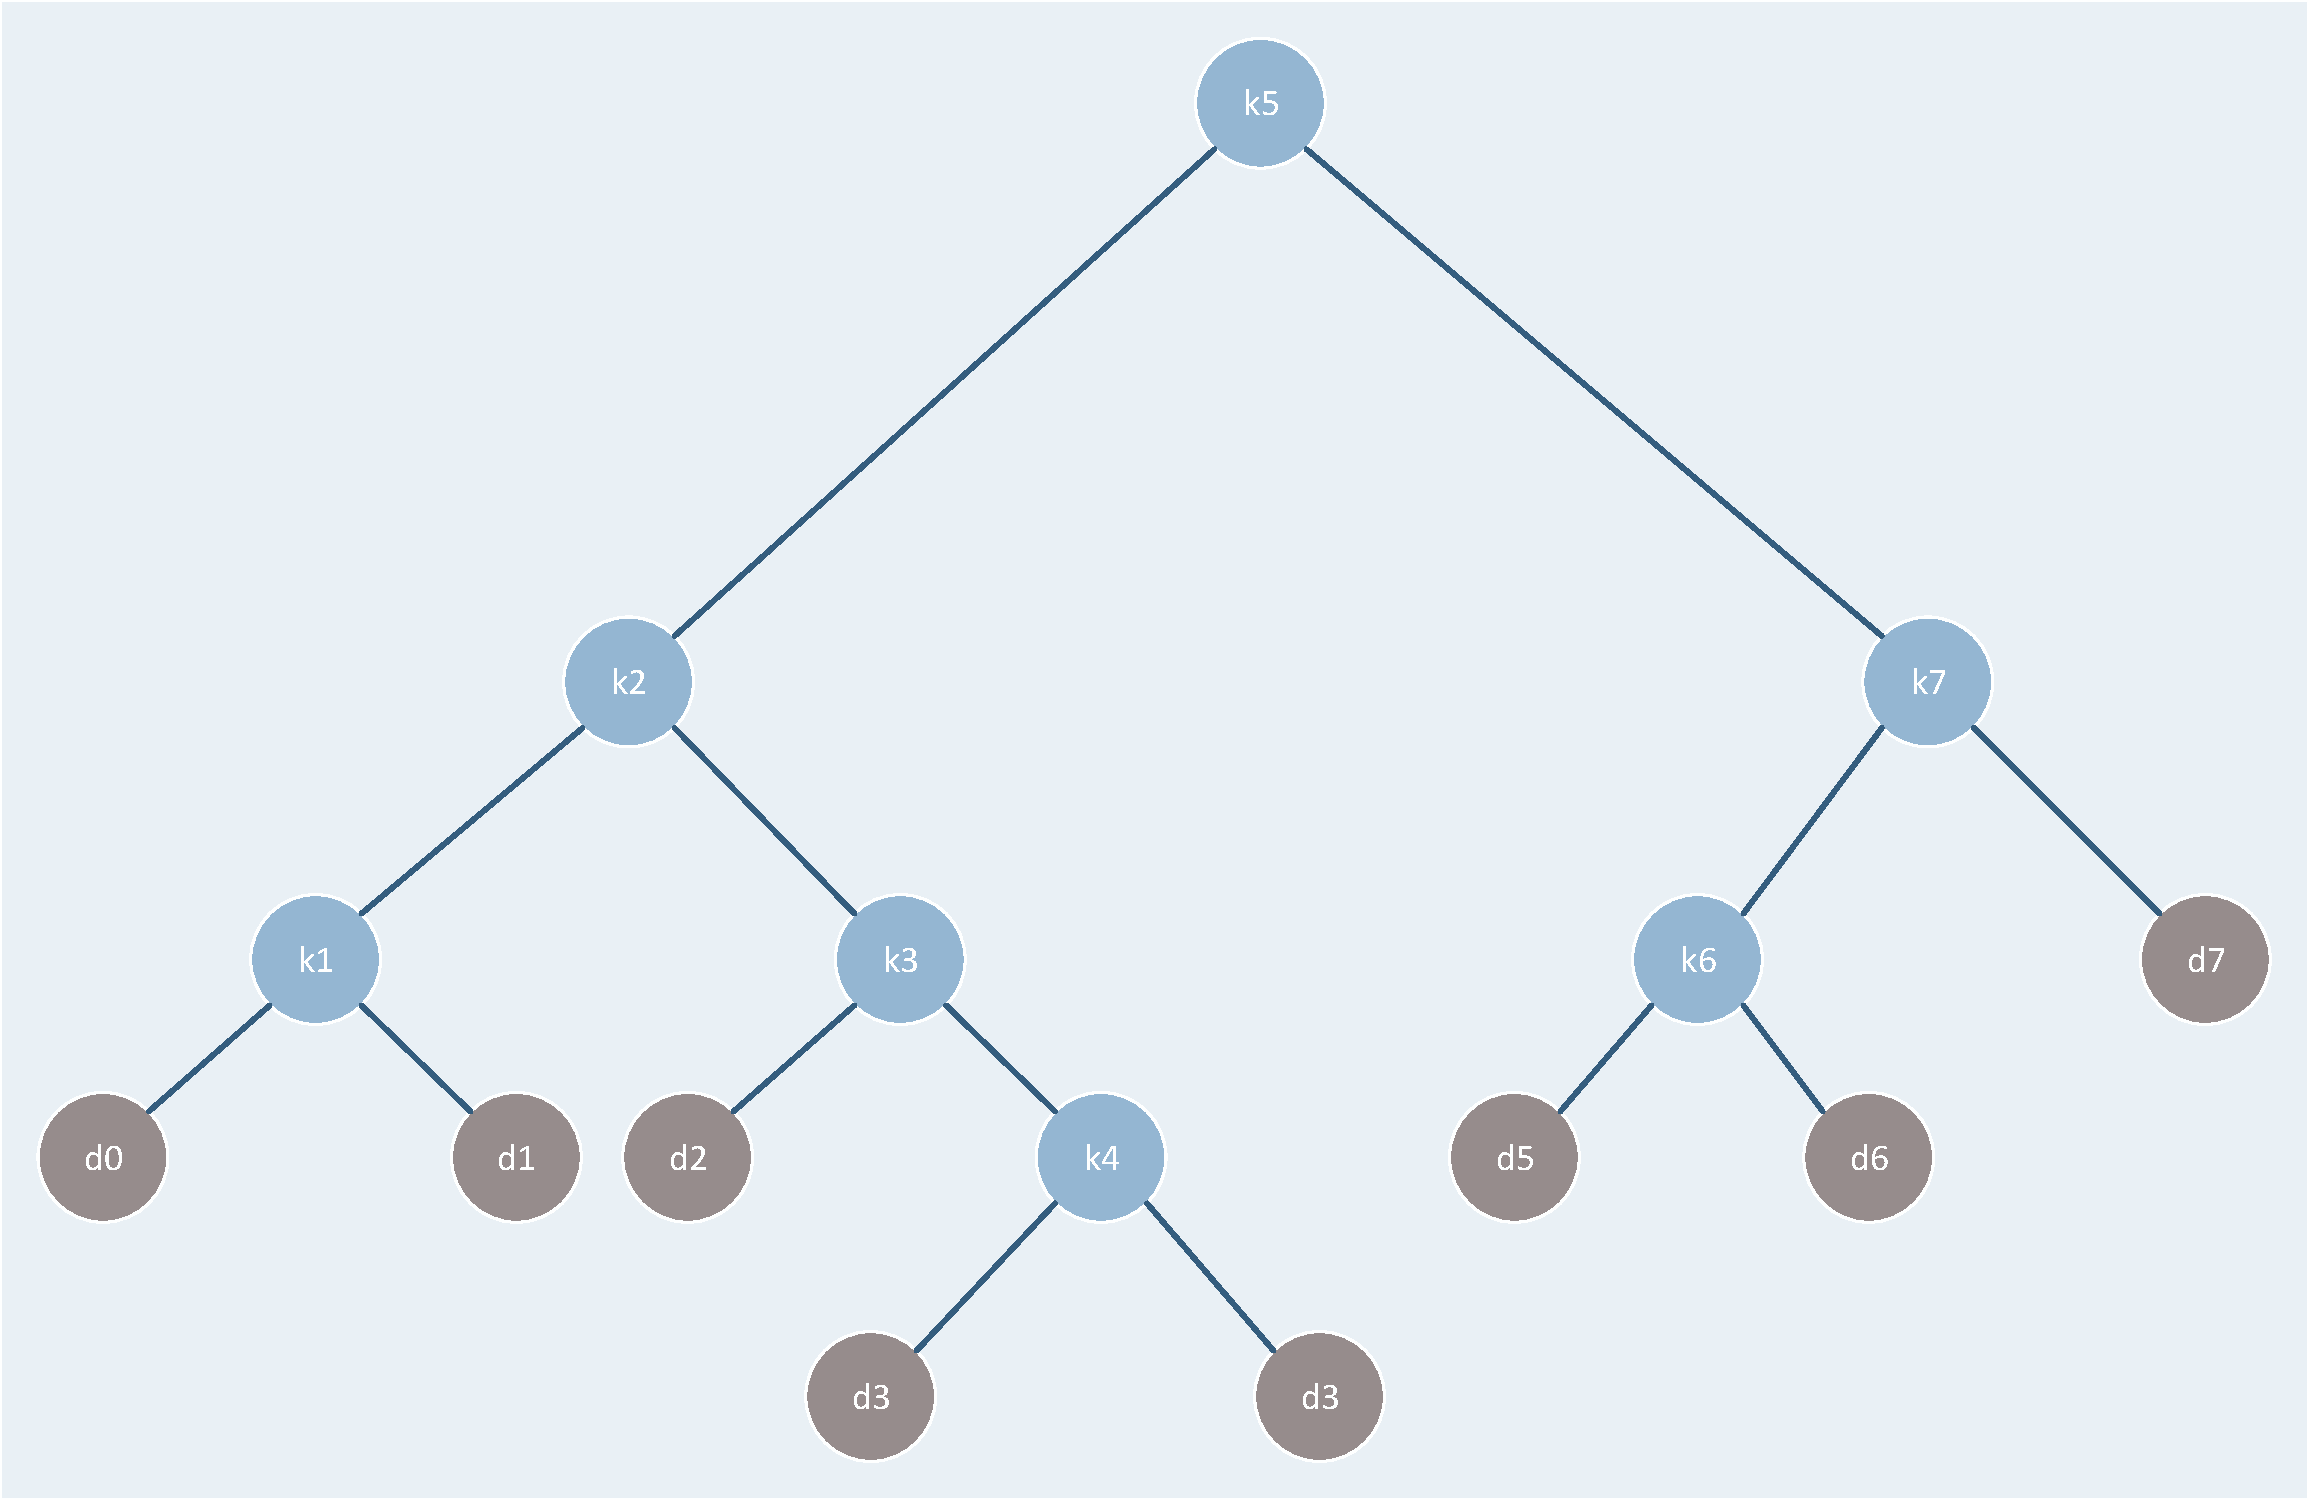
\includegraphics[width=0.8\textwidth]{Fig-Tree.pdf}
                        \caption{Optimal Binary Search Tree}\label{Fig-Tree}
                    \end{figure}
		            
		            \textbf{\textit{Explanation of the drawing process:}} 
		            
		            The drawing process could be divided into two parts: one is the \emph{drawing keys} and the other is \emph{drawing dummy keys.}
		            
		            \begin{enumerate}
		                \item [$k$:]
		                In terms of drawing $k$ nodes, I use a recursive method. Since element $e[i,j]$ stores the root of the subtree of $\{k_i,k_{i+1},\cdots,k_j\}$,the subtree of $\{k_i,k_{i+1},\cdots,k_{e[i,j]-1}\}$ is the left subtree of $k_{e[i,j]-1}$ and the subtree of $\{k_{e[i,j]+1},k_{e[i,j]+2},\cdots,k_{j}\}$ is the left subtree of $k_{e[i,j]-1}$, where $i<e[i,j]<j$. Such method could draw an optimal binary search tree of nodes $\{k_1,k_{2},\cdots,k_n\}$ if the input is $i=1$ and $j=n$.
		                
		                \item [$d$:]
		                The key point is to judge whether a key is a leaf of the binary search tree. Considering the property of the array $e$, if node $e[i,j]$ has no left subtree, $e[i,j]=i$ must be true.(Otherwise the subtree of $\{k_i,k_{i+1},\cdots,k_{e[i,j]-1}\}$ must contains at least one \emph{key} node)
		                Thus we could draw dummy keys by conditional branches. If $e[i,j]=i$, the left subtree of \emph{key} node $K_{e[i,j]}$ is a \emph{dummy node} $d_{e[i,j]-1}$. If $e[i,j]=j$, the right subtree of \emph{key} node $K_{e[i,j]}$ is a \emph{dummy node} $d_{e[i,j]}$.
		            \end{enumerate}

		        \end{enumerate} 
		    \end{solution}
		
		\item \textit{Dynamic Time Warping Distance.} \textbf{DTW} stretches the series along the time axis in a dynamic way over different
		portions to enable more effective matching. Let $D T W(i, j)$ be the optimal distance between the first $i$ and first $j$ elements of two time series $\bar{X}=\left(x_{1} \ldots x_{n}\right)$ and $\bar{Y}=\left(y_{1} \ldots y_{m}\right),$ respectively. Note that the two time series are of lengths $n$ and $m$, which may not be the same. Then, the value of $D T W(i, j)$ is defined recursively as follows:
		$$
		DTW(i, j)=\left|x_{i}- y_{j}\right|+\min(DTW(i, j-1), DTW(i-1, j), DTW(i-1, j-1))
		$$
		
		\begin{enumerate}
			\item Implement the proposed DTW algorithm in C/C++ and analyze the time complexity of your implementation. ({\color{blue}The framework Code-DTW.cpp is attached on the course webpage}). Two test cases have been given in the source code. 
			\item The window constraint imposes a minimum level $w$ of positional alignment between matched elements. The window constraint requires that $DTW(i, j)$ be computed only when $|i-j| \leq w$. Modify your code to add a window constraint and give the results of $ w=0 $ and $ w=1 $ on the two test cases. 
		\end{enumerate}
		    \begin{solution}
		    ~\\
		    \textbf{\textit{Explanation of vagueness:}}
		    \begin{enumerate}
		        \item [1.]\emph{Normalized distance} 
		        $$Normalized\ distance=\frac{\sum_{(i,j)\in \ path} DTW[i,j]}{Number\ of\ nodes\ in\ path}$$
		        \item [2.]\emph{The rule of window constraint condition}
		        
		        The sentence \textit{The window constraint requires that $DTW(i, j)$ be computed only when $|i-j| \leq w$.} in the question means that $DTW(i,j)$ does not exist and we have no idea computing it when $|i-j|\leq w$, so we could set $+\infty$ to $DTW(i,j)$ mathematically in such condition.
		    \end{enumerate}
		    \textbf{\textit{Result of the program:}}
		    \begin{figure}[htbp]
                \centering 
                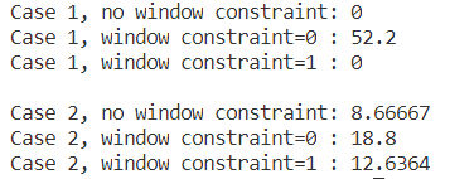
\includegraphics[width=0.6\textwidth]{Fig-Result2.pdf}
                \caption{Program Result}\label{Fig-Result}
            \end{figure}
            \\
            \\
		    \textbf{\textit{Time complexity analysis:}}
		    
		    The process of computing the \emph{time normalized distance} has three serial parts:

		        \textbf{Fill in the $DTW$ matrix:} The process only need a two-level for loop to traverse the $DTW$ matrix of size $n\times m$, so the time complexity of it is $\Theta(mn)$.
		        
		        \textbf{Identify the warping path:} The operation will trace from $D[n,m]$ back to $D[0,0]$. The worst case is that no step is diagonal, of which the time complexity is $O(m+n)$. As a result, the average time complexity will not exceed $O(m,n)$.
		        
		        \textbf{Calculate th time normalized distance:} The operation sums the $DTW$ value of each node in the path. The longest possible length of the path is $n+m-1$, so the worst time complexity is $O(m+n)$. The Average time complexity will not exceeds $O(m+n)$.
		        
		        \textbf{Conclusion}:
		        $$Time\ complexity=\Theta(mn)+2O(m+n)=\Theta(mn)$$
		        \\
		        \\
                \textbf{\textit{Modification of window constraint:}} 
                The two modifications of the source code is explained as \emph{comment} in the line $27-30$ and line $54-59$ of the file \emph{Code-DTW.cpp}. Screen shoots of the two comments are shown in  Fig.~\ref{Fig-Modification1}. and Fig.~\ref{Fig-Modification2}
                \begin{figure}[htbp]
                \centering 
                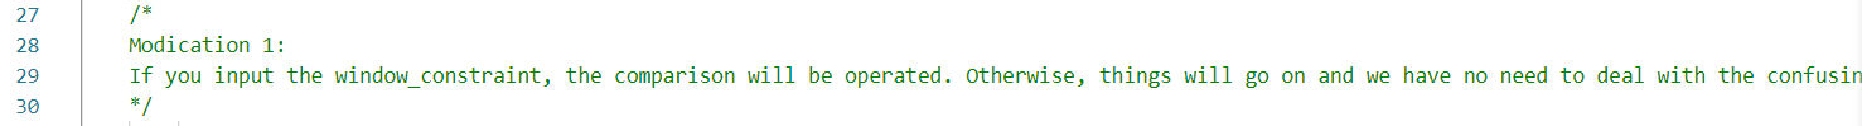
\includegraphics[width=0.8\textwidth]{Fig-Modification1.pdf}
                \caption{Screen shoot of modification 1}\label{Fig-Modification1}
                \end{figure}
                
                \begin{figure}[htbp]
                \centering 
                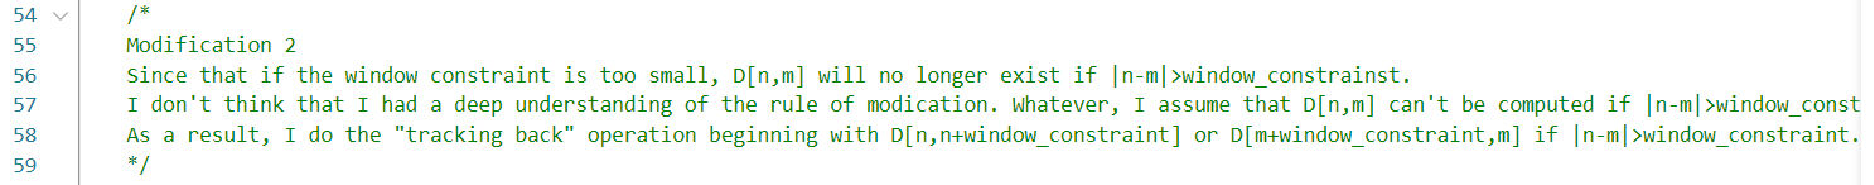
\includegraphics[width=0.8\textwidth]{Fig-Modification2.pdf}
                \caption{Screen shoot of modification 2}\label{Fig-Modification2}
                \end{figure}
		    \end{solution}
		
	\end{enumerate}
	
	\vspace{20pt}
	
	\textbf{Remark:} You need to include your .pdf and .tex and {\color{red}\emph{$2$}} source code files in your uploaded .rar or .zip file. Screenshots of test case results are acceptable.
	
	%========================================================================
\end{document}
